% -*- mode: noweb; noweb-default-code-mode: R-mode; -*-
%\VignetteIndexEntry{panelcn.mops: Manual for the R package}
%\VignetteDepends{panelcn.mops}
%\VignettePackage{panelcn.mops}
%\VignetteEngine{knitr::knitr}
%\VignetteKeywords{copy number analysis, mixture distribution, latent variables,
% Poisson distribution, EM algorithm, NGS, CNV, copy number variant}


\documentclass[article]{bioinf}\usepackage[]{graphicx}\usepackage[]{color}
%% maxwidth is the original width if it is less than linewidth
%% otherwise use linewidth (to make sure the graphics do not exceed the margin)
\makeatletter
\def\maxwidth{ %
  \ifdim\Gin@nat@width>\linewidth
    \linewidth
  \else
    \Gin@nat@width
  \fi
}
\makeatother

\definecolor{fgcolor}{rgb}{0.345, 0.345, 0.345}
\newcommand{\hlnum}[1]{\textcolor[rgb]{0.686,0.059,0.569}{#1}}%
\newcommand{\hlstr}[1]{\textcolor[rgb]{0.192,0.494,0.8}{#1}}%
\newcommand{\hlcom}[1]{\textcolor[rgb]{0.678,0.584,0.686}{\textit{#1}}}%
\newcommand{\hlopt}[1]{\textcolor[rgb]{0,0,0}{#1}}%
\newcommand{\hlstd}[1]{\textcolor[rgb]{0.345,0.345,0.345}{#1}}%
\newcommand{\hlkwa}[1]{\textcolor[rgb]{0.161,0.373,0.58}{\textbf{#1}}}%
\newcommand{\hlkwb}[1]{\textcolor[rgb]{0.69,0.353,0.396}{#1}}%
\newcommand{\hlkwc}[1]{\textcolor[rgb]{0.333,0.667,0.333}{#1}}%
\newcommand{\hlkwd}[1]{\textcolor[rgb]{0.737,0.353,0.396}{\textbf{#1}}}%

\usepackage{framed}
\makeatletter
\newenvironment{kframe}{%
 \def\at@end@of@kframe{}%
 \ifinner\ifhmode%
  \def\at@end@of@kframe{\end{minipage}}%
  \begin{minipage}{\columnwidth}%
 \fi\fi%
 \def\FrameCommand##1{\hskip\@totalleftmargin \hskip-\fboxsep
 \colorbox{shadecolor}{##1}\hskip-\fboxsep
     % There is no \\@totalrightmargin, so:
     \hskip-\linewidth \hskip-\@totalleftmargin \hskip\columnwidth}%
 \MakeFramed {\advance\hsize-\width
   \@totalleftmargin\z@ \linewidth\hsize
   \@setminipage}}%
 {\par\unskip\endMakeFramed%
 \at@end@of@kframe}
\makeatother

\definecolor{shadecolor}{rgb}{.97, .97, .97}
\definecolor{messagecolor}{rgb}{0, 0, 0}
\definecolor{warningcolor}{rgb}{1, 0, 1}
\definecolor{errorcolor}{rgb}{1, 0, 0}
\newenvironment{knitrout}{}{} % an empty environment to be redefined in TeX

\usepackage{alltt}


\usepackage{amsmath,amssymb}
\usepackage{hyperref}
\usepackage{float}
\usepackage[authoryear]{natbib}

\hypersetup{colorlinks=false,
    pdfborder=0 0 0,
    pdftitle={panelcn.MOPS - CNV detection tool for targeted NGS panel 
    data},
    pdfauthor={Gundula Povysil}}

\title{panelcn.MOPS - CNV detection tool for targeted NGS panel data}
\author{Verena Haunschmid and Gundula Povysil}
\affiliation{Institute of Bioinformatics, Johannes Kepler University
Linz\\Altenberger Str. 69, 4040 Linz, Austria\\
\email{povysil@bioinf.jku.at}}

\newcommand{\panelcnmops}{\texttt{panelcn.mops}}
\newcommand{\cnmops}{\texttt{cn.mops}}

\newcommand{\method}[1]{{\fontfamily{phv}\fontshape{rm}\selectfont #1}}
\newcommand{\R}{R}
\newcommand{\Real}{\mathbb{R}}

\renewcommand{\vec}[1]{\mathbf{#1}}

\setkeys{Gin}{width=0.55\textwidth}




\IfFileExists{upquote.sty}{\usepackage{upquote}}{}
\begin{document}




\newcommand{\cnmopsVersion}{0.1.4}
\manualtitlepage[Version \cnmopsVersion, \today]

%\section*{Scope and Purpose of this Document}
%
%This document is a user manual for the \R\ package \panelcn.mops.
%It is only meant as a gentle introduction into how to use the basic
%functions implemented in this package. Not all features of the \R\
%package are described in full detail. Such details can be obtained
%from the documentation enclosed in the \R\ package. Further note
%the following: (1) this is neither an introduction to CNV detection from NGS
%data; (2) this is not an introduction to \R.
%If you lack the background for understanding this manual, you first
%have to read introductory literature on these subjects.
%


\vspace{1cm}

\newlength{\auxparskip}
\setlength{\auxparskip}{\parskip}
\setlength{\parskip}{0pt}
\tableofcontents
\clearpage
\setlength{\parskip}{\auxparskip}

\newlength{\Nboxwidth}
\setlength{\Nboxwidth}{\textwidth}
\addtolength{\Nboxwidth}{-2\fboxrule}
\addtolength{\Nboxwidth}{-2\fboxsep}

\newcommand{\notebox}[1]{%
\begin{center}
\fbox{\begin{minipage}{\Nboxwidth}
\noindent{\sffamily\bfseries Note:} #1
\end{minipage}}
\end{center}}

\section{Introduction}
The \panelcnmops\ package is based on the
\cnmops\ package and allows to detect copy number variations (CNVs) from
targeted NGS panel data. Please visit
\url{http://www.bioinf.jku.at/software/panelcnmops/index.html} for additional
information.\par



\section{Getting started and quick start}

To load the package, enter the following in your \R\ session:
\begin{knitrout}
\definecolor{shadecolor}{rgb}{0.969, 0.969, 0.969}\color{fgcolor}\begin{kframe}
\begin{alltt}
\hlkwd{library}\hlstd{(panelcn.mops)}
\end{alltt}
\end{kframe}
\end{knitrout}

The whole pipeline will only take a few steps, if BAM files are available
(for read count matrices directly go to step 2):

\begin{enumerate}
\item Getting count windows from the BED file (also see Section \ref{s:input}).
\begin{knitrout}
\definecolor{shadecolor}{rgb}{0.969, 0.969, 0.969}\color{fgcolor}\begin{kframe}
\begin{alltt}
\hlstd{bed} \hlkwb{<-} \hlstr{"Genes_part.bed"}
\hlstd{countWindows} \hlkwb{<-} \hlkwd{getWindows}\hlstd{(bed)}
\end{alltt}
\end{kframe}
\end{knitrout}

\item Getting read counts from BAM file (also see Section \ref{s:input}).
\begin{knitrout}
\definecolor{shadecolor}{rgb}{0.969, 0.969, 0.969}\color{fgcolor}\begin{kframe}
\begin{alltt}
\hlstd{testfile} \hlkwb{<-} \hlstr{"SAMPLE1.bam"}
\hlstd{test} \hlkwb{<-} \hlkwd{countBamListInGRanges}\hlstd{(}\hlkwc{countWindows} \hlstd{= countWindows,}
                                \hlkwc{bam.files} \hlstd{= testfile,} \hlkwc{read.width} \hlstd{=} \hlnum{150}\hlstd{)}
\end{alltt}
\end{kframe}
\end{knitrout}

\item Running the algorithm (also see Section \ref{s:panelcn.mops}).
\begin{knitrout}
\definecolor{shadecolor}{rgb}{0.969, 0.969, 0.969}\color{fgcolor}\begin{kframe}
\begin{alltt}
\hlkwd{data}\hlstd{(panelcn.mops)}

\hlstd{selectedGenes} \hlkwb{<-} \hlkwd{c}\hlstd{(}\hlstr{"ATM"}\hlstd{)}

\hlstd{XandCB} \hlkwb{<-} \hlstd{test}
\hlkwd{elementMetadata}\hlstd{(XandCB)} \hlkwb{<-} \hlkwd{cbind}\hlstd{(}\hlkwd{elementMetadata}\hlstd{(XandCB),}
                                \hlkwd{elementMetadata}\hlstd{(control))}

\hlstd{resultlist} \hlkwb{<-} \hlkwd{runPanelcnMops}\hlstd{(XandCB,}
                            \hlkwc{testiv} \hlstd{=} \hlnum{1}\hlopt{:}\hlkwd{ncol}\hlstd{(}\hlkwd{elementMetadata}\hlstd{(test)),}
                            \hlkwc{countWindows} \hlstd{= countWindows,}
                            \hlkwc{selectedGenes} \hlstd{= selectedGenes)}
\end{alltt}
\end{kframe}
\end{knitrout}

\item Visualization of the detected CNV regions. For more information about
the result objects and visualization see Section \ref{s:results} and 
Section \ref{s:plot}.






\begin{knitrout}
\definecolor{shadecolor}{rgb}{0.969, 0.969, 0.969}\color{fgcolor}\begin{kframe}
\begin{alltt}
\hlstd{sampleNames} \hlkwb{<-} \hlkwd{colnames}\hlstd{(}\hlkwd{elementMetadata}\hlstd{(test))}
\hlstd{resulttable} \hlkwb{<-} \hlkwd{createResultTable}\hlstd{(}\hlkwc{result} \hlstd{= resultlist,} \hlkwc{XandCB} \hlstd{= XandCB,}
                                    \hlkwc{countWindows} \hlstd{= countWindows,}
                                    \hlkwc{selectedGenes} \hlstd{= selectedGenes,}
                                    \hlkwc{sampleNames} \hlstd{= sampleNames)}
\end{alltt}


{\ttfamily\noindent\itshape\color{messagecolor}{\#\# Calculating results for sample(s) SAMPLE1.bam}}

{\ttfamily\noindent\itshape\color{messagecolor}{\#\# Building table...}}

{\ttfamily\noindent\itshape\color{messagecolor}{\#\# Finished}}\begin{alltt}
\hlstd{(}\hlkwd{tail}\hlstd{(resulttable[[}\hlnum{1}\hlstd{]]))}
\end{alltt}
\begin{verbatim}
##         Sample Chr Gene                              Exon
## 57 SAMPLE1.bam  11  ATM ATM.E58.chr11.108216439.108216666
## 58 SAMPLE1.bam  11  ATM ATM.E59.chr11.108217975.108218123
## 59 SAMPLE1.bam  11  ATM ATM.E60.chr11.108224462.108224638
## 60 SAMPLE1.bam  11  ATM ATM.E61.chr11.108225507.108225632
## 61 SAMPLE1.bam  11  ATM ATM.E62.chr11.108235778.108235976
## 62 SAMPLE1.bam  11  ATM ATM.E63.chr11.108236021.108236266
##        Start       End   RC  medRC RC.norm medRC.norm lowQual
## 57 108216439 108216666  969  768.5     736        702        
## 58 108217975 108218123  375  301.0     285        276        
## 59 108224462 108224638  828  692.0     629        629        
## 60 108225507 108225632  701  550.0     533        533        
## 61 108235778 108235976 1373  793.0    1043        707        
## 62 108236021 108236266 1727 1018.5    1312        934        
##     CN
## 57 CN2
## 58 CN2
## 59 CN2
## 60 CN2
## 61 CN3
## 62 CN3
\end{verbatim}
\end{kframe}
\end{knitrout}



\begin{knitrout}
\definecolor{shadecolor}{rgb}{0.969, 0.969, 0.969}\color{fgcolor}\begin{kframe}
\begin{alltt}
\hlkwd{plotBoxplot}\hlstd{(}\hlkwc{result} \hlstd{= resultlist[[}\hlnum{1}\hlstd{]],} \hlkwc{sampleName} \hlstd{= sampleNames[}\hlnum{1}\hlstd{],}
            \hlkwc{countWindows} \hlstd{= countWindows,}
            \hlkwc{selectedGenes} \hlstd{= selectedGenes,} \hlkwc{showGene} \hlstd{=} \hlnum{1}\hlstd{)}
\end{alltt}
\end{kframe}
\end{knitrout}




\begin{figure}[H]
\begin{center}
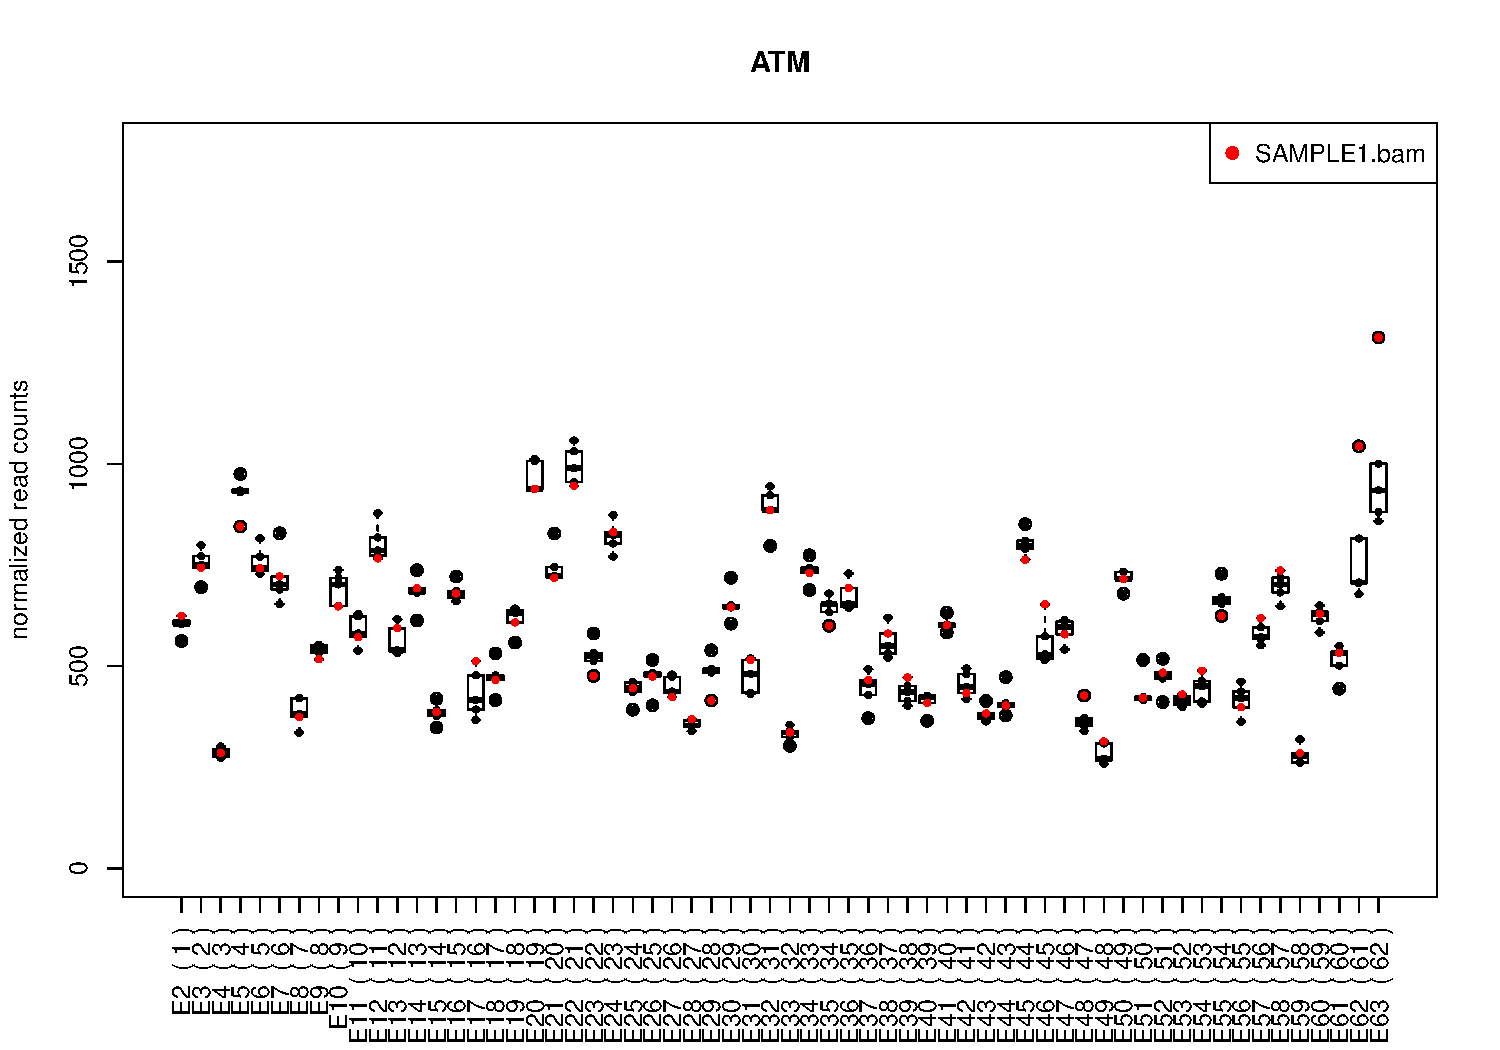
\includegraphics[angle=0,width= 0.9\columnwidth]{001.pdf}
\end{center}
\end{figure}
\end{enumerate}

\section{Input}
\label{s:input}
% \subsection{Read count matrices as input}
% Like \cnmops\ \panelcnmops\ does not require the data samples to be of any
% specific kind or structure. \cnmops\ only requires a {\em read count matrix},
% i.e., given $N$ data samples and $m$ genomic segments, this is an $m\times N$
% real- or integer-valued matrix $\mathbf{X}$,
% in which an entry $x_{ij}$ corresponds to the read count of sample $j$ in the
% $i$-th segment. E.g. in the following read count matrix sample three has
% $17$ reads in the second segment: $x_{23}=71$.
% 
% 
% \newlength{\mylen}
% \setlength{\mylen}{0.43cm}
% 
% \[\mathbf{X}= \begin{array}{c} \\ \mathrm{Segment\ 1} \\ \mathrm{Segment\ 2} 
% \\ \mathrm{Segment\ 3} \\ \mathrm{Segment\ 4}\\ \mathrm{Segment\ 5} \\
% \mathrm{Segment\ 6} \\ \hspace{0.2cm} \end{array}
% \begin{array}{c}
% \begin{array}{cccc}
% \mathrm{Sample\ 1} & \mathrm{Sample\ 2} & \mathrm{Sample\ 3} &
% \mathrm{Sample\ 4}\end{array}\\
% \left(\begin{array}{cccc}
% \hspace{\mylen}88\hspace{\mylen} & \hspace{\mylen}82\hspace{\mylen} &
% \hspace{\mylen}79\hspace{\mylen} & \hspace{\mylen}101\hspace{\mylen}\\
% 83 & 78 & 71 & 99\\
% 43 & 50 & 55 & 37\\
% 47 & 58 & 48 & 42 \\
% 73 & 86 & 95 & 91\\
% 92 & 90 & 80 & 71
% \end{array}\right) \\ \hspace{0.2cm}  \end{array}
% \]
% 
% 
% \panelcnmops\ can handle numeric and integer matrices or \verb+GRanges+ 
% objects, in which the read counts are stored as \verb+values+ of the object.
% 
% 
% 
% \subsection{BAM files as input}
% \label{s:bam}
The most widely used file format for aligned short reads is the Sequence
Alignment Map (SAM) format or in the compressed form the Binary Alignment Map
(BAM). \panelcnmops\ modifies the read count function \verb+countBamInGRanges+
from the \R\ package \texttt{exomeCopy} to extract read counts for a list of
BAM files.
The result object of the function can directly be used as input for
\panelcnmops.

The first step is to extract all ROIs that define the count windows from a 
BED file with the function \verb+getWindows+. 
\begin{knitrout}
\definecolor{shadecolor}{rgb}{0.969, 0.969, 0.969}\color{fgcolor}\begin{kframe}
\begin{alltt}
\hlstd{bed} \hlkwb{<-} \hlkwd{list.files}\hlstd{(}\hlkwd{system.file}\hlstd{(}\hlstr{"extdata"}\hlstd{,} \hlkwc{package} \hlstd{=} \hlstr{"panelcn.mops"}\hlstd{),}
                        \hlkwc{pattern} \hlstd{=} \hlstr{".bed$"}\hlstd{,} \hlkwc{full.names} \hlstd{=} \hlnum{TRUE}\hlstd{)}
\hlstd{countWindows} \hlkwb{<-} \hlkwd{getWindows}\hlstd{(bed)}
\end{alltt}


{\ttfamily\noindent\itshape\color{messagecolor}{\#\# naming without chr prefix chosen, but BED contains chr -> removing chr}}\end{kframe}
\end{knitrout}

The BED file should have the following structure:
\begin{knitrout}
\definecolor{shadecolor}{rgb}{0.969, 0.969, 0.969}\color{fgcolor}\begin{kframe}
\begin{verbatim}
## chr1 45794947 45795140 MUTYH.E16.chr1.45794947.45795140
## chr1 45796157 45796260 MUTYH.E15.chr1.45796157.45796260
## chr1 45796823 45797037 MUTYH.E14.chr1.45796823.45797037
## chr1 45797061 45797259 MUTYH.E13.chr1.45797061.45797259
## chr1 45797302 45797552 MUTYH.E12.chr1.45797302.45797552
## chr1 45797664 45797789 MUTYH.E11.chr1.45797664.45797789
\end{verbatim}
\end{kframe}
\end{knitrout}

While the first 3 columns list chromosome name, start and end position, the 
fourth column needs to start with the gene name. Additional information in the 
fourth column needs to be separated with a dot and may include the exon number 
and further information. By default the "chr" prefix of the chromosome name is 
removed if present. This can be changed by setting the {\tt chr} parameter to 
TRUE. If a mismatch of chromosome naming between the \verb+countWindows+ object 
and the BAM files is detected, the naming convention of the BAM file is chosen.


In the second step RCs are generated from the BAM files. The read.width 
parameter reflects the typical length of the reads that should be counted.

\begin{knitrout}
\definecolor{shadecolor}{rgb}{0.969, 0.969, 0.969}\color{fgcolor}\begin{kframe}
\begin{alltt}
\hlstd{testbam} \hlkwb{<-} \hlkwd{list.files}\hlstd{(}\hlkwd{system.file}\hlstd{(}\hlstr{"extdata"}\hlstd{,} \hlkwc{package} \hlstd{=} \hlstr{"panelcn.mops"}\hlstd{),}
                        \hlkwc{pattern} \hlstd{=} \hlstr{".bam$"}\hlstd{,} \hlkwc{full.names} \hlstd{=} \hlnum{TRUE}\hlstd{)}
\hlstd{test} \hlkwb{<-} \hlkwd{countBamListInGRanges}\hlstd{(}\hlkwc{countWindows} \hlstd{= countWindows,}
                                \hlkwc{bam.files} \hlstd{= testbam,} \hlkwc{read.width} \hlstd{=} \hlnum{150}\hlstd{)}
\end{alltt}


{\ttfamily\noindent\itshape\color{messagecolor}{\#\# Processing SAMPLE1.bam ... 1 / 1}}

{\ttfamily\noindent\itshape\color{messagecolor}{\#\# finished processing samples}}\end{kframe}
\end{knitrout}

In \verb+test+ you have now stored the genomic segments (left of the
$\mid$'s) and the read counts (right of the $\mid$'s):
\begin{knitrout}
\definecolor{shadecolor}{rgb}{0.969, 0.969, 0.969}\color{fgcolor}\begin{kframe}
\begin{alltt}
\hlstd{(test)}
\end{alltt}
\begin{verbatim}
## GRanges object with 370 ranges and 1 metadata column:
##         seqnames               ranges strand   | SAMPLE1.bam
##            <Rle>            <IRanges>  <Rle>   |   <integer>
##     [1]        1 [45794947, 45795140]      *   |         637
##     [2]        1 [45796157, 45796260]      *   |         384
##     [3]        1 [45796823, 45797037]      *   |         414
##     [4]        1 [45797061, 45797259]      *   |         361
##     [5]        1 [45797302, 45797552]      *   |         482
##     ...      ...                  ...    ... ...         ...
##   [366]        2 [48032018, 48032197]      *   |         618
##   [367]        2 [48032726, 48032877]      *   |         206
##   [368]        2 [48033312, 48033528]      *   |         572
##   [369]        2 [48033560, 48033821]      *   |         735
##   [370]        2 [48033887, 48034030]      *   |         678
##   -------
##   seqinfo: 11 sequences from an unspecified genome; no seqlengths
\end{verbatim}
\end{kframe}
\end{knitrout}

\section{runPanelcnMops}
\label{s:panelcn.mops}
The actual copy number analysis is done with the function \verb+runPanelcnMops+.
The function requires a \verb+GRanges+ object of the RCs of test and control 
samples as well as the \verb+countWindows+ object used to extract these RCs.
Optional parameters include a vector that indicates which samples to regard as 
test samples (default = c(1)), a vector of the names of the genes of interest 
(by default all genes are of interest), parameters for normalizing the RCs, 
a vector of expected fold changes for the copy number classes and a minimal 
median RC over all samples to exclude low coverage ROIs.

\begin{knitrout}
\definecolor{shadecolor}{rgb}{0.969, 0.969, 0.969}\color{fgcolor}\begin{kframe}
\begin{alltt}
\hlkwd{data}\hlstd{(panelcn.mops)}

\hlstd{XandCB} \hlkwb{<-} \hlstd{test}
\hlkwd{elementMetadata}\hlstd{(XandCB)} \hlkwb{<-} \hlkwd{cbind}\hlstd{(}\hlkwd{elementMetadata}\hlstd{(XandCB),}
                                \hlkwd{elementMetadata}\hlstd{(control))}
\hlstd{resultlist} \hlkwb{<-} \hlkwd{runPanelcnMops}\hlstd{(XandCB,} \hlkwc{countWindows} \hlstd{= countWindows)}
\end{alltt}
\end{kframe}
\end{knitrout}



\section{Results}
\label{s:results}
The function \verb+runPanelcnMops+ returns a list of objects of the S4 class 
CNVDetectionResult, one CNVDetectionResult object per test sample. 
The structure of the CNVDetectionResult object can be listed by calling
\begin{knitrout}
\definecolor{shadecolor}{rgb}{0.969, 0.969, 0.969}\color{fgcolor}\begin{kframe}
\begin{alltt}
\hlstd{(}\hlkwd{str}\hlstd{(resultlist[[}\hlnum{1}\hlstd{]]))}
\end{alltt}
\end{kframe}
\end{knitrout}

To get
detailed information on which data are stored in such objects, enter
\begin{knitrout}
\definecolor{shadecolor}{rgb}{0.969, 0.969, 0.969}\color{fgcolor}\begin{kframe}
\begin{alltt}
\hlkwd{help}\hlstd{(CNVDetectionResult)}
\end{alltt}
\end{kframe}
\end{knitrout}



The CNVs per individual are stored in the slot \verb+integerCopyNumber+:
\begin{knitrout}
\definecolor{shadecolor}{rgb}{0.969, 0.969, 0.969}\color{fgcolor}\begin{kframe}
\begin{alltt}
\hlkwd{integerCopyNumber}\hlstd{(resultlist[[}\hlnum{1}\hlstd{]])[}\hlnum{1}\hlopt{:}\hlnum{5}\hlstd{]}
\end{alltt}
\begin{verbatim}
## GRanges object with 5 ranges and 5 metadata columns:
##       seqnames               ranges strand | SAMPLE1.bam
##          <Rle>            <IRanges>  <Rle> |    <factor>
##   [1]        1 [45794947, 45795140]      * |         CN2
##   [2]        1 [45796157, 45796260]      * |         CN2
##   [3]        1 [45796823, 45797037]      * |         CN2
##   [4]        1 [45797061, 45797259]      * |         CN2
##   [5]        1 [45797302, 45797552]      * |         CN2
##       SAMPLE4.bam SAMPLE3.bam SAMPLE6.bam SAMPLE2.bam
##          <factor>    <factor>    <factor>    <factor>
##   [1]         CN2         CN2         CN2         CN2
##   [2]         CN2         CN2         CN2         CN2
##   [3]         CN2         CN2         CN2         CN2
##   [4]         CN2         CN2         CN2         CN2
##   [5]         CN2         CN2         CN2         CN2
##   -------
##   seqinfo: 11 sequences from an unspecified genome; no seqlengths
\end{verbatim}
\end{kframe}
\end{knitrout}



The function \verb+createResultTable+ summarizes all relevant information for 
user selected genes of interest in a list of tables with one table per test 
sample:


\begin{knitrout}
\definecolor{shadecolor}{rgb}{0.969, 0.969, 0.969}\color{fgcolor}\begin{kframe}
\begin{alltt}
\hlstd{sampleNames} \hlkwb{<-} \hlkwd{colnames}\hlstd{(}\hlkwd{elementMetadata}\hlstd{(test))}
\hlstd{resulttable} \hlkwb{<-} \hlkwd{createResultTable}\hlstd{(}\hlkwc{result} \hlstd{= resultlist,} \hlkwc{XandCB} \hlstd{= XandCB,}
                                    \hlkwc{countWindows} \hlstd{= countWindows,}
                                    \hlkwc{selectedGenes} \hlstd{= selectedGenes,}
                                    \hlkwc{sampleNames} \hlstd{= sampleNames)}
\end{alltt}


{\ttfamily\noindent\itshape\color{messagecolor}{\#\# Calculating results for sample(s) SAMPLE1.bam}}

{\ttfamily\noindent\itshape\color{messagecolor}{\#\# Building table...}}

{\ttfamily\noindent\itshape\color{messagecolor}{\#\# Finished}}\begin{alltt}
\hlstd{(}\hlkwd{tail}\hlstd{(resulttable[[}\hlnum{1}\hlstd{]]))}
\end{alltt}
\begin{verbatim}
##         Sample Chr Gene                              Exon
## 57 SAMPLE1.bam  11  ATM ATM.E58.chr11.108216439.108216666
## 58 SAMPLE1.bam  11  ATM ATM.E59.chr11.108217975.108218123
## 59 SAMPLE1.bam  11  ATM ATM.E60.chr11.108224462.108224638
## 60 SAMPLE1.bam  11  ATM ATM.E61.chr11.108225507.108225632
## 61 SAMPLE1.bam  11  ATM ATM.E62.chr11.108235778.108235976
## 62 SAMPLE1.bam  11  ATM ATM.E63.chr11.108236021.108236266
##        Start       End   RC  medRC RC.norm medRC.norm lowQual
## 57 108216439 108216666  969  768.5     736        702        
## 58 108217975 108218123  375  301.0     285        276        
## 59 108224462 108224638  828  692.0     629        629        
## 60 108225507 108225632  701  550.0     533        533        
## 61 108235778 108235976 1373  793.0    1043        707        
## 62 108236021 108236266 1727 1018.5    1312        934        
##     CN
## 57 CN2
## 58 CN2
## 59 CN2
## 60 CN2
## 61 CN3
## 62 CN3
\end{verbatim}
\end{kframe}
\end{knitrout}

The table contains one line per Region Of Interest (ROI) with information about 
the RCs of the test sample ("RC"), 
the median RCs of all control samples ("medRC"), 
the normalized RCs of the test sample ("RC.norm"), 
the median of the normalized RCs of all control samples ("medRC.norm"), 
as well as the estimated CN ("CN"). 
Additionally, in the column "lowQual" low quality ROIs are flagged.



\section{Visualization of results}
\label{s:plot}
\panelcnmops\ contains a plotting function that visualizes the normalized RCs 
of the samples analyzed as boxplots:

\begin{center}
\begin{knitrout}
\definecolor{shadecolor}{rgb}{0.969, 0.969, 0.969}\color{fgcolor}\begin{kframe}
\begin{alltt}
\hlkwd{plotBoxplot}\hlstd{(}\hlkwc{result} \hlstd{= resultlist[[}\hlnum{1}\hlstd{]],} \hlkwc{sampleName} \hlstd{= sampleNames[}\hlnum{1}\hlstd{],}
            \hlkwc{countWindows} \hlstd{= countWindows,}
            \hlkwc{selectedGenes} \hlstd{= selectedGenes,} \hlkwc{showGene} \hlstd{=} \hlnum{1}\hlstd{)}
\end{alltt}
\end{kframe}
\end{knitrout}


\begin{figure}[H]
\begin{center}
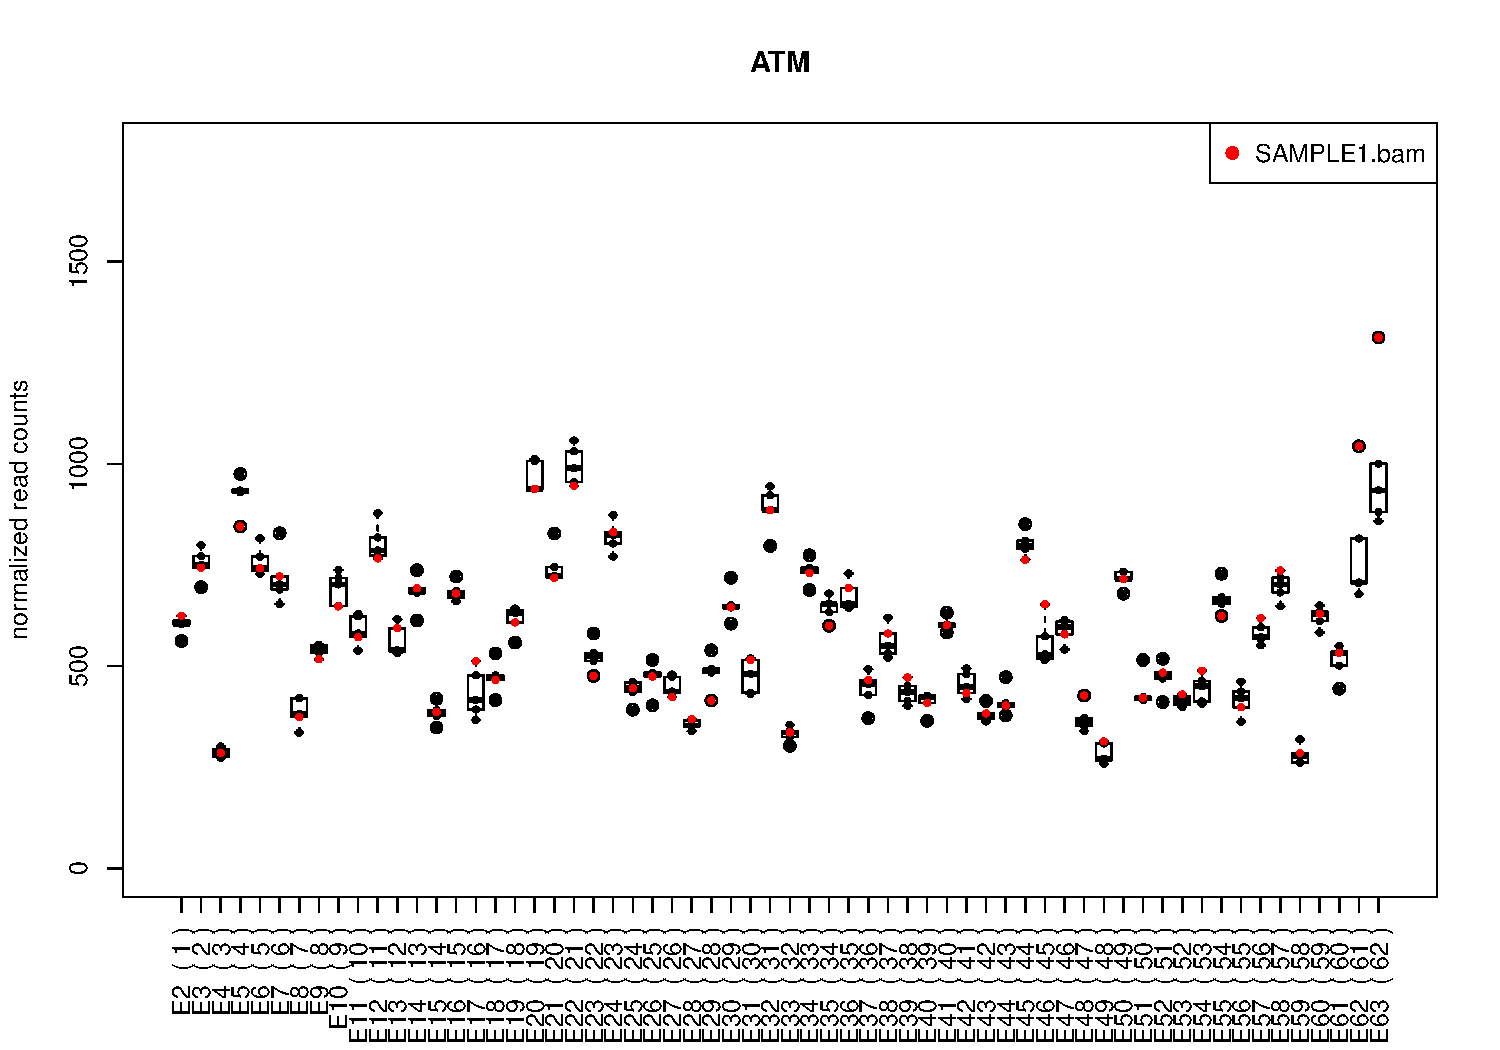
\includegraphics[angle=0,width= 0.9\columnwidth]{001.pdf}
\end{center}
\end{figure}
\end{center}

The function expects a single CNVDetectionResult object as input together with 
the name of the test sample, the countWindows used, as well as a vector with 
the names of the genes of interest and an integer specifying which of the 
genes of interest to plot.

\section{Quality control}

The panelcn.MOPS algorithm includes different quality control metrics. 1) ROIs 
are excluded if their median read count (RC) across all samples does not exceed 
a user defined threshold (default: 30), additionally a warning message is 
displayed. 2) ROIs are marked as "low quality" in the result table if their RCs 
show a high variation across all samples. 3) Samples with a median RC across 
all exons lower than 0.55 times the median of all samples are considered as low 
quality. 4) For each ROI the ratio between the normalized RCs of each sample 
compared to the median across all samples is calculated. Samples that show a 
high variation in these RC ratios are also flagged as low quality. Low quality 
samples are excluded if they are control samples which leads to a warning 
message. If a test sample is of low quality, only a warning message is 
displayed. 

\section{Adjusting sensitivity and specificity}
The default parameters of the \panelcnmops\ algorithm were optimized on a data 
set of targeted NGS panel data with the aim of detecting CNVs ranging in size 
from part of a ROI to whole genes. However, you might want to adjust 
sensitivity and specificity to your specific needs.

The parameter that influences sensitivity and specificity the most is {\tt I}, 
the vector of expected fold changes of the copy number classes. The default for 
\panelcnmops\, c(0.025, 0.57, 1, 1.46, 2), leads to a higher sensitivity 
compared to the default of \cnmops\ which is c(0.025, 0.5, 1, 1.5, 2). 
Increasing the values for CN0 and CN1 further and decreasing the values for 
CN3 and CN4 may help to improve the sensitivity, a change in the other 
direction may increase the specificity.

Additional parameters that can be tuned to improve the results are the 
different normalization parameters: {\tt normType}, {\tt sizeFactor}, 
{\tt qu}, {\tt quSizeFactor}, and {\tt norm}.




% \clearpage


\section{How to cite this package}

If you use this package for research that is published later, you are kindly
asked to cite it as follows:
\citep{Klambauer:11}.

To obtain Bib\TeX\ entries of the reference, you can enter the following
into your R session:
\begin{knitrout}
\definecolor{shadecolor}{rgb}{0.969, 0.969, 0.969}\color{fgcolor}\begin{kframe}
\begin{alltt}
\hlkwd{toBibtex}\hlstd{(}\hlkwd{citation}\hlstd{(}\hlstr{"cn.mops"}\hlstd{))}
\end{alltt}
\end{kframe}
\end{knitrout}


\bibliographystyle{natbib}
\bibliography{cnv}


\end{document}
